%!TEX encoding = UTF-8

\chapter{Affordances, Gestures and Language}
\label{chap:gestures}

In this chapter, we present a computational model (see Fig.~\ref{fig:gestures:gestures_lang_computational_model}) that combines object affordances with communication, and we show the benefits of such an approach in cognitive robotic systems.

\begin{figure}[h]
\newcommand{\myscaleaffmodels}{0.7}
\centering
\begin{tikzpicture}[scale=\myscaleaffmodels, every node/.style={transform shape}]
\montesanoAE
\montesanoO
\saponaroGestRecBox
\salviW
\end{tikzpicture}
\caption{Computational model of affordances with gestures and language.}
\label{fig:gestures:gestures_lang_computational_model}
\end{figure}

We consider two aspects of communication: nonverbal (i.e., body gestures) and verbal (i.e., language).
It is worth exploring both of these modalities in robots, as means for providing them the skills to engage in sociality and collaboration with humans.
In other words, communication is useful for becoming social\footnote{A social robot is ``[a robot that is] able to communicate and interact with us, understand and even relate to us, in a personal way. [It] should be able to understand us and itself in social terms''~\cite{breazeal:2002:dsr}.}.
By incorporating communication aspects into a cognitive robotic system, we permit the leap from ego-centric behavior~(where the robot explores its surrounding world) to a social one~(where the robot perceives the actions of other agents and links them to its own actions).

Regarding nonverbal communication, we focus on human \emph{gestures} perceived with vision sensors.
We developed a gesture recognizer for manipulative hand gestures.
This recognizer receives a sequence of camera images depicting a person making manipulative gestures (these images contain the \emph{gesture feature} inputs), and it produces a probability distribution
over the gesture being recognized as output\footnote{Implementation details about the gesture recognition model will be given in Appendix~\ref{chap:gesture_recognition}. \label{footnote:link_to_appendix_gest_rec}}.

We embed the gesture recognizer into a computational model of object affordances, permitting to extend previous works (\cite{salvi:2012:smcb}, see also Sec.~\ref{sec:background:previous_works:aff_language}).
With our combination of affordances and gestures we show that, after having acquired knowledge of its surrounding environment from autonomous exploration, a humanoid robot can generalize this knowledge to the case when it observes another agent~(human partner) performing the same motor actions previously executed by the robot during training.
This is the shift from reasoning purely about actions performed by the robot itself~(ego-centric phase) to reasoning about actions performed by external human users~(social phase).

We also incorporate \emph{verbal language} capabilities into the model, motivated by the observation that \hh{} cooperation is greatly facilitated and influenced by human language~\cite{mueller:2000:psych}, therefore language description skills can benefit \hr{} cooperation.
In addition, having the verbal language component in our computational model allows us to visualize the results produced by the robot from a different angle.

Throughout this chapter, we use the following \emph{terminology}, in accordance to a review by Aggarwal on human activity recognition~\cite{aggarwal:2011}. \label{para:action_terminology}
Human activities can be categorized into different levels with increasing level of complexity.
\emph{Gestures} are elementary movements of a person's body part, and are the atomic components describing the meaningful motion of a person.
\emph{Actions} are single-person activities that may be composed of multiple gestures organized temporally, such as walking or waving.
\emph{Interactions} are activities that involve two or more persons and/or objects.

We make the code and data from this chapter publicly available%
\footnote{\url{https://github.com/gsaponaro/tcds-gestures}: code from \cite{saponaro:2019:language}. \label{footnote:tcds-gestures_url}% end footnote
} in the interest of reproducibility.

This chapter is the subject of the following publications:
\listPublicationsGestures

The outline of this chapter is as follows.
Sec.~\ref{sec:gestures:motivation} gives motivations for building models that jointly consider object affordances and communication~(nonverbal and verbal).
Sec.~\ref{sec:gestures:related} lists related works from the robotic literature implementing this fusion.
Sec.~\ref{sec:gestures:approach} presents our proposed approach for combining object affordances, nonverbal communication~(gestures), and verbal language.
In Sec.~\ref{sec:gestures:results} we report the experimental results,
and finally in Sec.~\ref{sec:gestures:conclusions} we draw our conclusions and possible future extensions.

\section{Motivation}
\label{sec:gestures:motivation}

Communication is defined as ``a process by which information is exchanged between individuals through a common system of symbols, signs, or behavior''\footnote{\url{https://www.merriam-webster.com/dictionary/communication}}.
In this section, we motivate why combining object affordances with communication (gestures and language) can be beneficial in cognitive robotic systems, as already hinted in the beginning of this chapter and in Sec.~\ref{sec:motivation:affordances}.

The common system of symbols existing between individuals during communication can be encoded by nonverbal aspects~(e.g., body gestures) as well as verbal ones~(i.e., natural human language).
Both nonverbal gestures and verbal words have specific motivations to be incorporated in robot perception algorithms and robot cognitive capabilities.
By relying on a gesture recognizer,
we augment the computational affordance model of Sec.~\ref{sec:background:previous_works:montesano} with gestures, permitting the shift from reasoning about actions performed by the robot itself~(ego-centric phase) to reasoning about actions performed by external users~(social phase).
In addition, we incorporate language into the model, allowing to estimate the probability of words given other observed variables.
This kind of reasoning over language is useful for human interpretability, because it allows to generate verbal descriptions of experimental data.
It also shows how our model can exhibit semantic language properties:
the choice of relevant words to describe a scene,
the choice of synonyms,
and of congruent/incongruent conjunctions.

We now give some motivations for incorporating gestures and words, respectively, in cognitive robotic systems.

\emph{Gestures} expose the role of physical movement in communication and interaction\footnote{%
Human gestures can be \emph{static} or \emph{dynamic}.
During static gestures, body joints do not move: examples are pointing, or displaying a number with the fingers.
Instead, in dynamic gestures, body joints move: for example during waving and clapping.
In the case of sign languages, a gesture can have both static and dynamic elements.
In this chapter \emph{we draw our attention to dynamic gestures}, which, due to their rapidly evolving nature, are particularly relevant in the manipulative scenarios that we consider, introduced in Sec.~\ref{sec:platform:scenario}. \label{footnote:static_dynamic_gestures}}% end footnote
.
Humans learn to use gestures during their first year of age, even before they learn to speak~\cite{tomasello:2007:cd}.
Psychology has studied how humans interact with body gestures for many activities and purposes~\cite{mcneill:1996,messing:1999}, including: greeting, leaving, showing agreement or disagreement, threatening, emphasizing a spoken sentence, physically pointing at something or someone.
In this chapter, we employ a gesture recognition model capable of recognizing the manipulative gesture made by a person probabilistically\footref{footnote:link_to_appendix_gest_rec}.

\emph{Verbal language} is another fundamental aspect of human communication that is useful to model in machines, particularly for the collaborative aspect.
A child acquires the skill of coordinating with peers or adult caregivers in shared problem-solving activities and social games (therefore, to \emph{collaborate}) around the second year of life~\cite{brownell:2006:childdev}: this is achieved not only by mere behavioral coordination, but also by employing communicative strategies~\cite{melis:2010:rstb} and by continuously observing partners' actions~\cite{ramnani:2004:natureneuro}.

Even though social robots
are becoming common in domestic and public environments, \hr{} teams still lag behind \hh{} teams in terms of effectiveness.
For robots, interpreting the actions of others and learning to describe them verbally~(for effective cooperation) is challenging.
One reason is that we cannot possibly model all the imaginable verbal cues that can take place during \hri, due to the richness of language and the high variability of the real world outside of structured research laboratories and factories.
A viable alternative is to have robots that \emph{learn} world elements and properties of language~\cite{iwahashi:2007:hri}, and the ability to link these verbal elements with other skills, such as other perceptual modalities~(e.g., vision of objects and other agents) and manipulation abilities~(e.g., grasping objects and placing them in order to achieve a goal)~\cite{steels:2003:trendscogsci}.

\begin{figure}
\centering
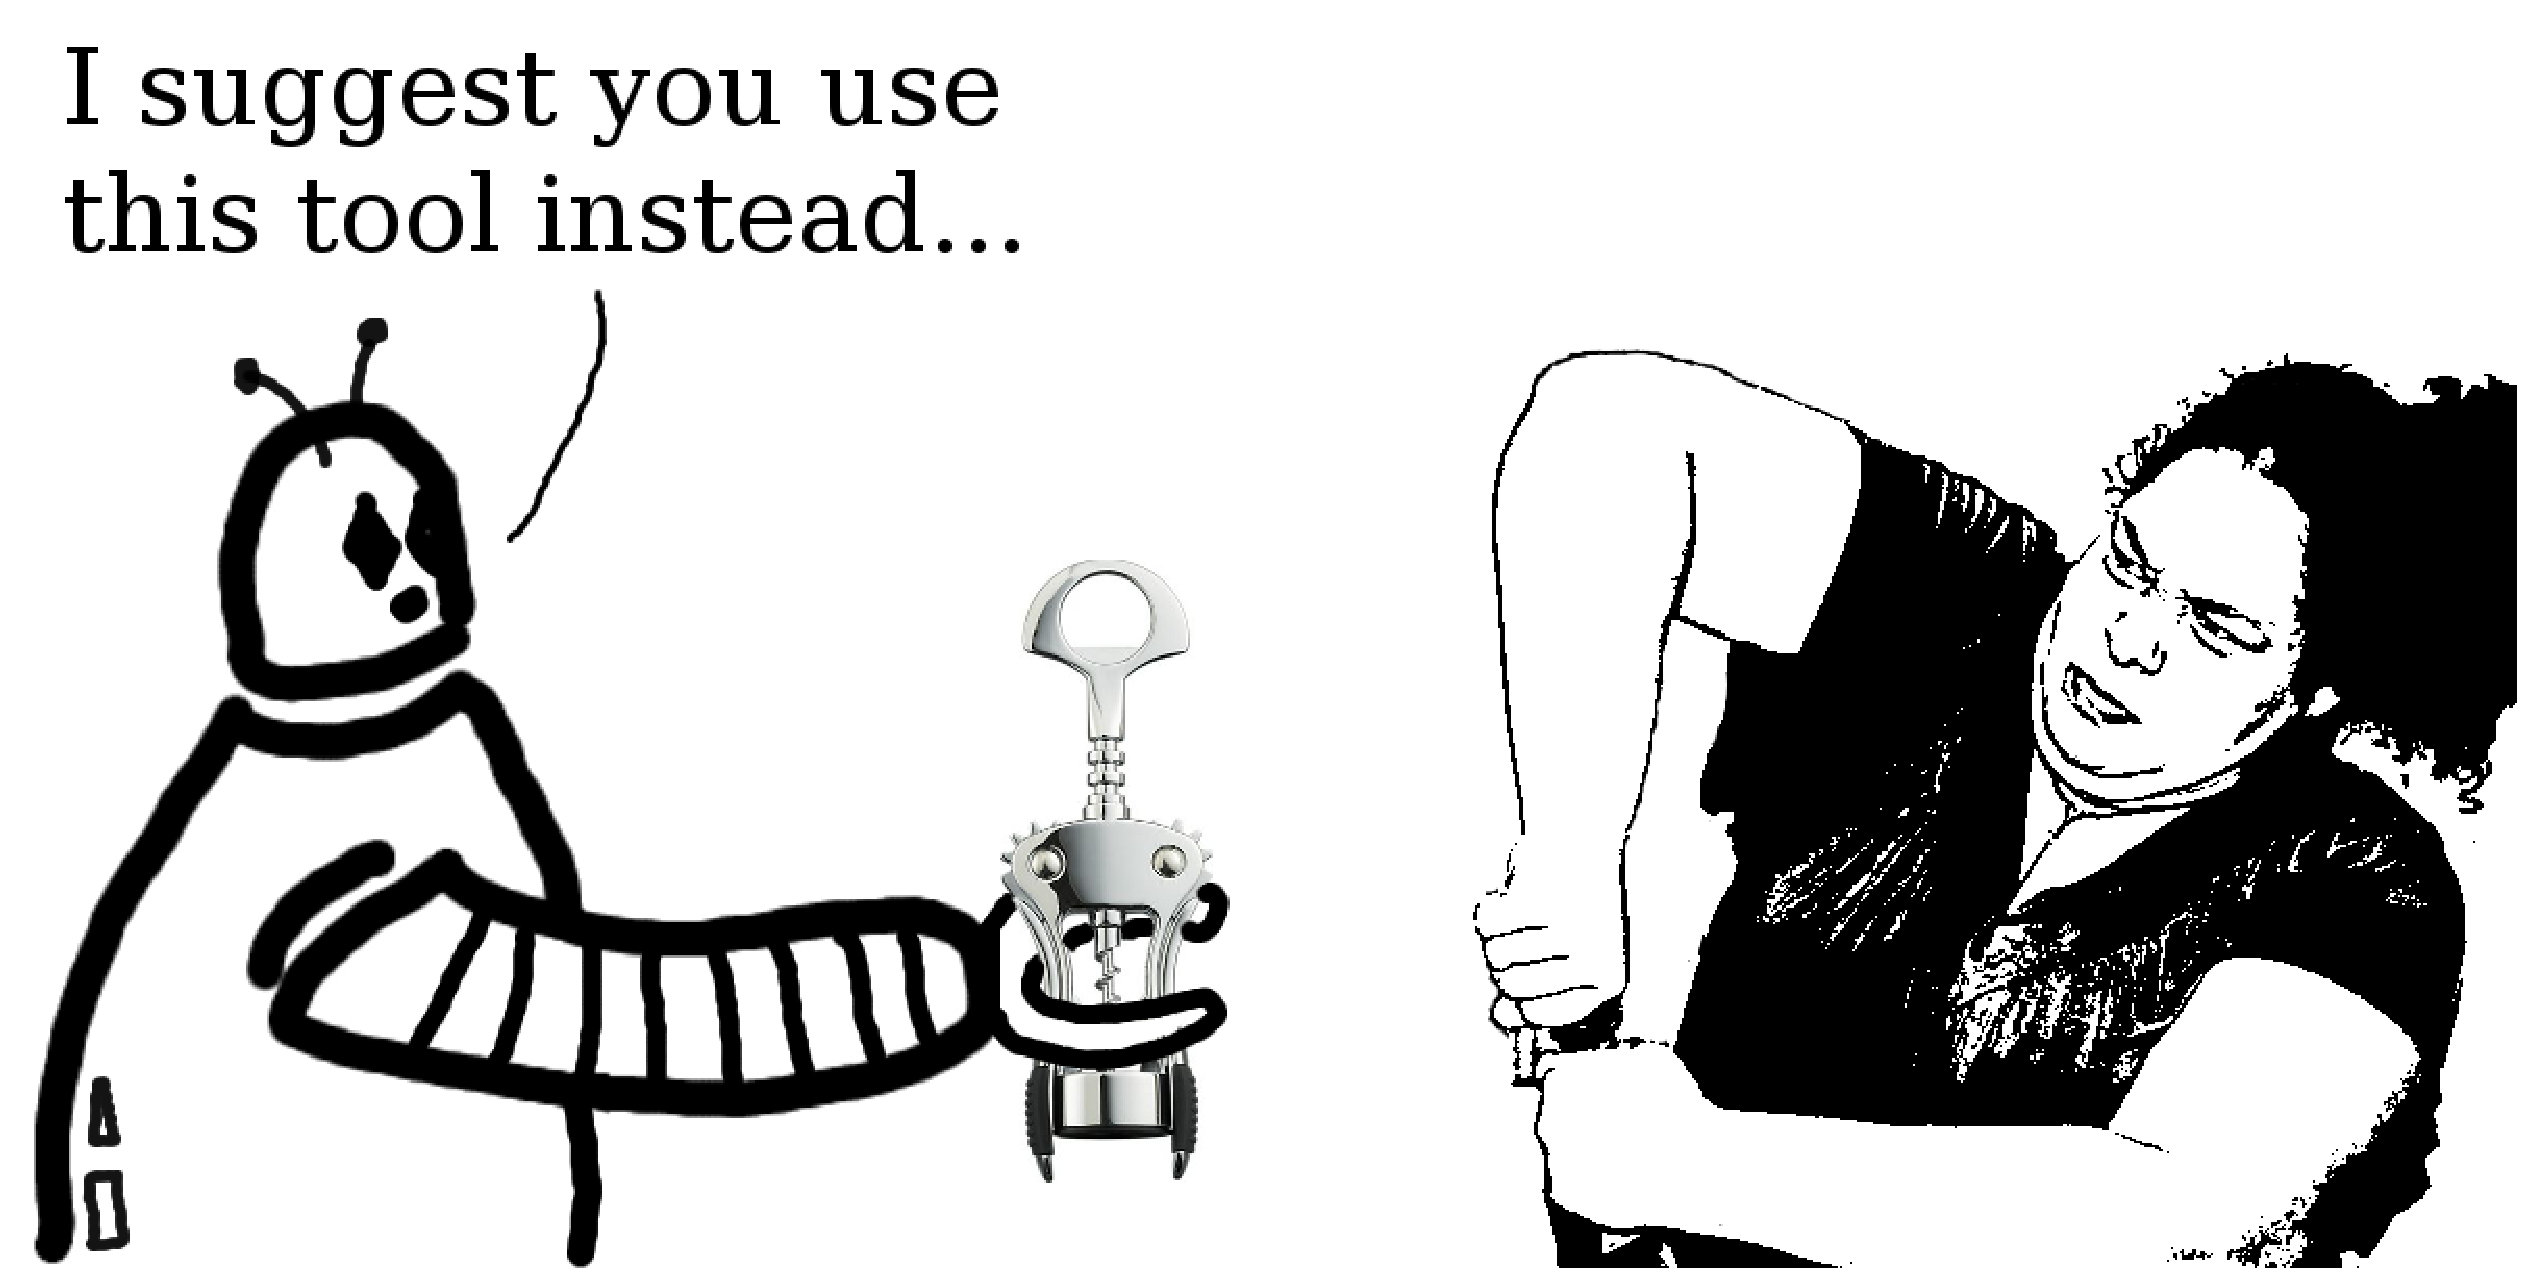
\includegraphics[width=0.9\textwidth]{robot_helper}
\caption[Proof of concept of a robot recognizing a human struggling while opening a bottle: the robot intervenes, providing help.]{Proof of concept of a robot~(left) recognizing a human struggling while opening a bottle~(right): the robot intervenes, providing help.
Picture elaborated from~\url{http://flic.kr/p/b8bbYZ} with permission from the original owner.}
\label{fig:robot_helper}
\end{figure}

A key motivation for using the above-mentioned sources of information~(object affordances, words, gestures) in robot algorithms, is to support \emph{activity recognition} of human agents.
For example, this is useful for revising the belief that a certain action occurred, given the observed effects of the human action onto physical objects (correction of action estimation).
In addition, a robot can anticipate the effects when the action has only been partially observed (early action recognition).
Equipping robots with these prediction capabilities allows them to anticipate effects before action completion, thus enabling interactions between human and robot to be uninterrupted and natural.

In turn, action recognition and prediction abilities serve:
(i)~to predict what is going to happen,
(ii)~to understand the \emph{motivation} beyond the others' action (mental simulation), and
(iii)~to provide feedback or commentary by an automated (possibly robotic) system.
Fig.~\ref{fig:robot_helper} sketches an example of these uses.
Inherent in this motivation is the leap from an ego-centric phase to a social one, permitting agents to reason about the actions of others, and to describe them verbally.
In this chapter, we illustrate our implementation of this process.

\section{Related Work}
\label{sec:gestures:related}

This section describes works that are related to the scope of this chapter, that is, the combination of object affordances with communication~(nonverbal and verbal) in cognitive robotic systems.

First, in Sec.~\ref{sec:gestures:related:salvi} we describe the model by Salvi in greater detail than in Ch.~\ref{chap:background}.
That work is the building block that this chapter extends.
Then, in Sec.~\ref{sec:gestures:related:other} we go through other works in the literature that use robot affordances and communication.

\subsection{Affordances and Language}
\label{sec:gestures:related:salvi}

In Sec.~\ref{sec:background:previous_works:aff_language}, we have introduced the \AffWords{} model by Salvi \cite{salvi:2012:smcb}.

Recall that Salvi proposes a joint model to learn robot affordances \emph{together with word meanings}.
It uses a Bayesian probabilistic framework to allow a robot to ground the basic world behavior and verbal descriptions associated to it, as shown in Fig.~\ref{fig:montesano_setup} on p.~\pageref{fig:montesano_setup} and Fig.~\ref{fig:salvi_setup} on p.~\pageref{fig:salvi_setup}.
The data used for learning such a model is obtained from robot manipulation experiments.
Each experiment is associated with a number of alternative verbal descriptions uttered by two human speakers according to a pre-defined grammar, for a total of \num{1270}~recordings.

Note, however, that in~\cite{salvi:2012:smcb} no grammar was used during the learning phase:
the speech recognizer used as a frontend to the spoken descriptions is based on a loop of words with no grammar, and the \AffWords{} model is based on a bag-of-words assumption, where only the presence or absence of each word in the description is considered.

The data in Salvi's work is acquired from a robot's \emph{ego-centric perspective}, meaning that the robot learns a model by interacting with the environment by self-exploration (see also Sec.~\ref{sec:motivation:devrob} and Sec.~\ref{sec:platform:scenario}), and then it reasons about its own actions.

\begin{figure}
  \tikzstyle{dashedgroup06} = [rectangle, draw, inner sep=0.6cm, dashed, rounded corners, black]
    \centering
    \begin{tikzpicture}
      % single nodes
      \node[affnode] (g1) {$g_1$};
      \node[affnode, right of=g1] (g2) {$g_2$};
      \node[right of=g2] (gdots) {$\dots$};
      \node[group, fit=(g1) (g2) (gdots),label=above:Gesture Features] (gestures) {};
      \node[affnode, below of=gestures] (actions) [below=1cm] {Actions};
      \node[affnode, right of=actions] (f1) [right=1.6cm] {$f_1$};
      \node[affnode, right of=f1] (f2) {$f_2$};
      \node[right of=f2] (fdots) {$\dots$};
      \node[affnode, below of=f1] (e2) [below=0.7cm] {$e_2$};
      \node[affnode, left of=e2] (e1) {$e_1$};
      \node[right of=e2] (edots) {$\dots$};
      \node[wordnode, below of=e1] (w1)  [below=0.7cm] {$w_1$};
      \node[wordnode, right of=w1] (w2) {$w_2$};
      \node[right of=w2] (wdots) {$\dots$};
      % groups
      \node[group, fit=(f1) (f2) (fdots),label=above:Object Features] (features) {};
      \node[group, fit=(e1) (e2) (edots),label=above:Effects] (effects) {};
      \node[group, fit=(w1) (w2) (wdots),label=above:Words] (words) {};
      \node[dashedgroup06, fit=(actions) (features) (effects) (words),label={[shift={(0:2.2)}]above:\AffWords{} model}]{};
      % arrows
      \draw[affarrow] (actions) -- ([xshift=-30pt]effects.north);
      \draw[affarrow] (actions) to [out=260,in=150] (words.west);
      \draw[affarrow] (features) -- ([xshift=20pt]effects.north);
      \draw[affarrow] ([xshift=20pt]features.south) to [out=280,in=30] (words.east);
      \draw[affarrow] ([xshift=30pt]effects.south) -- ([xshift=30pt]words.north);
      % extra
      \draw[affarrow] (actions) -- (gestures);
      \node[dashedgroup06, fit=(actions) (gestures),label=above:Gesture/Action recognition]{};
    \end{tikzpicture}
  \caption[Abstract representation of the probabilistic dependencies in our model which integrates affordances, gestures and language.]{Abstract representation of the probabilistic dependencies in our model which integrates affordances, gestures and language.
  See also Table~\ref{tab:salvi:bnsymb}.}
    \label{fig:gestures:full_model}
\end{figure}

\begin{table}
    \centering
    \caption[Symbolic variables of the \AffWords{} \acl{BN}.]{Symbolic variables of the \AffWords{} \acl{BN} (from~\cite{salvi:2012:smcb}), with the corresponding discrete values obtained from clustering during robot exploration of the environment.
    We call \emph{word variables} the booleans of the last row, whereas we call \emph{affordance variables} all the other symbols.
    See also Fig.~\ref{fig:gestures:full_model}.}
    \label{tab:salvi:bnsymb}
    \begin{tabular}{cp{3.7cm}l}
    \toprule
    symbol & name: description     & values \\
    \midrule
    $a$ & Action: motor action          & grasp, tap, touch \\
    \midrule
    $f_1$ & Color: object color   & blue, yellow, green1, green2 \\
    $f_2$ & Size: object size     & small, medium, big \\
    $f_3$ & Shape: object shape    & sphere, box \\
    \midrule
    $e_1$ & ObjVel: object velocity & slow, medium, fast \\
    $e_2$ & HandVel: robot hand velocity & slow, fast \\
    $e_3$ & ObjHandVel: relative \objecthand{} velocity & slow, medium, fast \\
    $e_4$ & Contact: object hand contact & short, long \\
    \midrule
    $w_1$--$w_{49}$ & presence of each word in the verbal description & true, false \\
    \bottomrule
    \end{tabular}
\end{table}

In this \AffWords{} model, the world behavior is defined by random variables, following the probabilistic machinery introduced in Ch.~\ref{chap:background}.
Table~\ref{tab:salvi:bnsymb} presents a list of variables and their possible values.

All variables are discrete or are discretized from continuous sensory variables through clustering in a preliminary learning phase.

Note that the name of the possible values have been assigned by the researchers arbitrarily to the clusters, for the sake of making the results more human-interpretable.
However, the robot has no prior knowledge about the meaning of these clusters nor about their order, in case they correspond to ordered quantities.

The variables can be divided according to their use: affordance variables and word variables.
Affordance variables are actions variables $A = \{a\}$, object feature variables $F=\{f_1, f_2, \dots\}$, and effect variables $E=\{e_1, e_2, \dots\}$.
Word variables are $W = \{w_1, w_2, \dots\}$.

To simplify the notation, let us call
\begin{align*}
X &= \{A, F, E, W\} \\
  &= \{a, f_1, f_2, \dots, e_1, e_2, \dots, w_1, w_2, \dots\}
\end{align*}
the set of affordance and word variables.
Consequently, the relationships between words and concepts are expressed by the joint probability distribution~$p(X) = p(A, F, E, W)$ of actions, object features, effects, and words in the spoken utterance.

This joint probability distribution,
illustrated by the dashed box labeled \AffWords{} model of Fig.~\ref{fig:gestures:full_model},
is estimated by the robot in an ego-centric way through interaction with the environment.
The dependency structure and the model parameters are estimated by the robot in an ego-centric way through interaction with the environment.
As a consequence, \emph{during learning, the robot knows \apriori{} what action it is performing with certainty, and the variable~$A$ assumes a deterministic value}.
During inference, the probability distribution of the variable~$A$ can be inferred from evidence on the other variables.
For example, if the robot is asked to make a spherical object roll, it will be able to select the action tap as most likely to obtain the desired effect, based on previous experience.

There is no one-to-one correspondence between affordance nodes and words in~\cite{salvi:2012:smcb}.
Each word is connected with many affordance nodes, that constitute the word's significant (for example, the word ``ball'' is not only connected to the shape object feature, but also to action and effect).

The lack of correspondence between affordance nodes and words was partly emerging from the natural variability that is inherent in the way humans describe situations in spoken words.
It was also a design choice, because in that work the authors wanted to prove that the model was not merely able to recover simple \wordmeaning{} associations, but was able to cope with more natural spoken utterances.
Consequently, in the spoken descriptions:
(i)~there are many synonyms for the same concept: for instance, cubic objects are called ``box'', ``square'' or ``cube''. Also, actions and effects are described using different tenses (``is grasping'', ``grasped'', ``has (just) grasped'');
(ii)~different affordance variable values may have the same associated verbal description, e.g., two color clusters corresponding to different shades of green are both referred to as ``green'';
(iii)~finally, many affordance variable values have no direct description: for example, the object velocity and \objecthand{} velocity~(slow, medium, fast), or the \objecthand{} contact~(short, long) are never described directly, and need to be inferred from the situation.

The \AffWords{} model does not account for the concepts of parts of speech, verb tenses or \emph{temporal aspects} explicitly.
For example, the words ``is'', ``grasping'', ``has'', ``grasped'', ``just'', and so on, are initially completely equivalent to the model, which has no prior information about what verbs, adjectives or nouns are, nor about similarity between words.
It is only through the association with the other robot observations that the model realizes that ``grasping'' has the same meaning as ``grasped''\footnote{The model of~\cite{salvi:2012:smcb} has no concept of past, present and future, and cannot distinguish between tenses.}.
The following three phrases, which were used interchangeably in the experiments by \cite{salvi:2012:smcb}, are mapped to exactly the same meaning, after learning:
(i)~``is grasping'',
(ii)~``has grasped'',
(iii)~``grasped''.
Note that the model \emph{per~se} would be fully capable to distinguish between those phrases, provided that they were used in different situations, which however was not the case in the experimental data.

The above assumption
of knowing the action with certainty during learning,
is relaxed in the proposed approach presented further down in this chapter, in Sec.~\ref{sec:gestures:approach}, by extending the model to the observation of external~(human) agents.
In doing this extension, we introduce a \emph{social perspective} where the robot reasons about other agents.

\subsection{Other Works}
\label{sec:gestures:related:other}

A few works have studied the potential coupling between learning robot affordances and \emph{language grounding} (where grounding refers to linking the symbolic nature of language with the sensorimotor experience of a robot).
The union of robot affordances with language grounding gives new skills to cognitive robots, such as:
creation of categorical concepts from multimodal association obtained by grasping and observing objects, while listening to partial verbal descriptions~\cite{nakamura:2009:iros,araki:2012:iros},
learning the association of spoken words with sensorimotor experience~\cite{morse:2016:cogsci}, linking language with sensorimotor representations~\cite{stramandinoli:2016:icdl}, or carrying out complex tasks~(which require \emph{planning} of a sequence of actions) expressed in natural language instructions to a robot.
The planning aspect will be the topic of Ch.~\ref{chap:poeticon++_case_study}.

In other works, both object-directed action recognition in external agents~\cite{koppula:2013:ijrr} and the incorporation of language in \hr{} systems~\cite{harnad:1990,matuszek:2014:aaai} have received ample attention, for example using the concept of \emph{intuitive physics}~\cite{lake:2017:bbs,gao:2018:acl} to be able to predict outcomes from real or simulated interactions with objects.

DeepMind and Google published a method~\cite{santoro:2017:relational_reasoning} to perform relational reasoning on images, i.e., a system that learns to reflect about entities and their mutual relations, with the ability of providing answers to questions such as ``Are there any rubber things that have the same size as the yellow metallic cylinder?''.
That work is very powerful from the point of view of cognitive systems, vision and language.
Our approach is different because
(i)~we focus on \emph{robotic} cognitive systems, including manipulation and the uncertainties inherent to robot vision and control, and
(ii)~we follow the developmental paradigm and the embodiment hypothesis~(see Sec.~\ref{sec:motivation:devrob}), meaning that, leveraging the fact that a human and a humanoid produce actions with similar effects, we relate words with the robot's \emph{sensorimotor} experience, rather than sensory only~(purely images-to-text).

\section{Proposed Approach}
\label{sec:gestures:approach}

In this section, we explain our approach for combining object affordances with communication~(nonverbal and verbal) in cognitive robotic systems.
This combination builds upon the intuition that a robot can use its previously-acquired knowledge of the world~(e.g., motor actions, objects properties, physical effects, verbal descriptions) to those situations where it observes a human agent performing familiar actions in a shared \hr{} scenario.

\subsection{Staged Developmental Process}
\label{sec:gestures:approach:stages}

Our method is a staged developmental process from a self-centered, individualistic learning, to socially aware learning.
This transition happens gradually in subsequent phases.

In the first phase, the system engages in manipulation activities with objects in its environment (following Montesano's approach, as described in Sec.~\ref{sec:background:previous_works:montesano}).
The robot learns object affordances by associating object properties, actions and the corresponding effects.

In a second phase, the robot interacts with a human who uses spoken language to describe the robot's activities (following Salvi's approach, as described in Sec.~\ref{sec:gestures:related:salvi}).
Here, the robot interprets the meaning of the words, grounding them in the \actionperception{} experience acquired so far.
Although this phase can already be considered \emph{social} for the presence of a human \emph{narrator}, it is still self-centered, because the robot is still learning how to interpret its own actions.

\begin{figure*}
  \centering
  \subfloat[][Grasp: moving the hand towards an object vertically, then grasping and lifting it.]{
    \resizebox{\linewidth}{!}{
      \includegraphics{grasp-00000169}
      \includegraphics{grasp-00000170}
      \includegraphics{grasp-00000171}
      \includegraphics{grasp-00000173}
      \includegraphics{grasp-00000177}
      \includegraphics{grasp-00000180}
    } % end resizebox
    \label{fig:gestures:human_action_examples:grasp}
  } % end subfloat

  \subfloat[][Tap: moving the hand towards an object laterally then touching it, causing a motion effect.]{
    \resizebox{\linewidth}{!}{
      \includegraphics{tap-00000109}
      \includegraphics{tap-00000110}
      \includegraphics{tap-00000112}
      \includegraphics{tap-00000114}
      \includegraphics{tap-00000116}
      \includegraphics{tap-00000117}
    } % end resizebox
    \label{fig:gestures:human_action_examples:tap}
  } % end subfloat

  \subfloat[][Touch: moving the hand towards an object vertically, touching it~(without grasping), then retracting the hand.]{
    \resizebox{\linewidth}{!}{
      \includegraphics{touch-00000196}
      \includegraphics{touch-00000197}
      \includegraphics{touch-00000198}
      \includegraphics{touch-00000200}
      \includegraphics{touch-00000202}
      \includegraphics{touch-00000203}
    } % end resizebox
    \label{fig:gestures:human_action_examples:touch}
  } % end subfloat
  \caption{Examples of human manipulative actions from the point of view of the robot.}
  \label{fig:gestures:human_action_examples}
\end{figure*}

In the last phase, which is our contribution, the system turns to observing human actions of a similar nature as the ones explored in the first phases.
We consider three \emph{manipulative gestures}, displayed in Fig.~\ref{fig:gestures:human_action_examples}, corresponding to physical actions performed by an agent onto objects on a table, in a similar fashion as in Sec.~\ref{sec:platform:scenario}.
The robot reuses the experience acquired in the first phases to interpret the new observations between its own actions and the actions performed by the human.
In this phase, human movements are interpreted using the experience acquired so far, and they are incorporated into the model using a gesture recognizer\footref{footnote:link_to_appendix_gest_rec}.

\subsection{Combining Affordances and Communication}
\label{sec:gestures:approach:affgest}

Starting from the \AffWords{} computational model by Salvi \cite{salvi:2012:smcb},
we propose a way to fuse two sources of information~(about the self and about others) in a fully probabilistic manner.
This addition allows to perform fine-grained types of inferences and reasoning, by doing predictions over affordances and words when observing another agent with uncertainty.

In extending Salvi's model, we relax the assumption (described in Sec.~\ref{sec:gestures:related:salvi}) that the action is known during the learning phase.
That assumption is acceptable when the robot learns through self-exploration and interaction with the environment, but must be relaxed if the robot needs to generalize the acquired knowledge through the observation of another~(human) agent.
We estimate the action performed by a human user during a \hr{} collaborative task, by employing a human gesture recognition algorithm\footref{footnote:link_to_appendix_gest_rec}.
This provides two advantages.
First, we can infer the executed action during training.
Second, at testing time we can merge the action information obtained from gesture recognition with the information about affordances.

To permit the transfer from robot self-centered knowledge to human knowledge to work, we assume that the \emph{same actions}, performed on objects with the \emph{same properties}, cause the \emph{same effects} and are described by the \emph{same words}.
In other terms, all of the variables under consideration, listed in Tab.~\ref{tab:salvi:bnsymb}, are the link between robot and human.

In our formulation and in our implementation, we will hinge on the existence of the discrete action variable, the value of which is known to the robot in the ego-centric phase of learning, but must be inferred when observing human actions.

The \emph{gesture recognition model} (that will be fully detailed in Appendix~\ref{chap:gesture_recognition})
is based on a statistical algorithm called \ac{HMM}: therefore, we denote the probabilities obtained by the gesture recognizer as~$\phmm(\cdot)$.
The input of this model is a sequence of~$T$ gesture feature vectors (the sequence going from image frame~$1$ to image frame~$T$), which we define as~$G_1^T$.
Thus, $\phmm(A \given G_1^T)$ denotes the probability distribution over the actions recognized by this model, given gesture features from~$1$ to~$T$.
For example, for a certain input we can obtain that $\phmm(A \given G_1^T)$ corresponds to the following action probabilities summing up to one: grasp~$0.8$, tap~$0.15$, touch~$0.05$.

We define the \AffWords{} model as $\pbn(A, F, E, W)$.
Our goal is to combine the information from $\pbn(A, F, E, W)$ and $\phmm(A \given G_1^T)$ into a single probabilistic model $\pcomb(A, F, E, W \given G_1^T)$, that is, the joint probability of all the affordance and word variables, given that we observe a certain action performed by the human.

The two models can be combined by having the gesture recognizer (Gesture \acp{HMM}) provide a posterior distribution to the \ac{BN}.
The posterior distribution represents a probabilistic or soft decision~\cite{pan:2006:ictai}, as opposed to a deterministic hard decision (which would consider only the top result with full confidence, and would be in fact a less general case, that we described in \cite{saponaro:2017:glu}).

Recall from Sec.~\ref{sec:gestures:related:salvi} that we call $X = \{A, F, E, W\}$ the set of affordance and word variables~$\{a, f_1, f_2, \dots, e_1, e_2, \dots, w_1, w_2, \dots\}$.
During inference, we have a (possibly empty) set of observed variables~$\xobs \subseteq X$, and a set of variables $\xinf \subseteq X$ on which we wish to perform the inference.
In order for the inference to be non-trivial, it must be~$\xobs \cap \xinf = \varnothing$, that is, we should not observe any inference variable.
According to the \ac{BN} alone, without the gesture recognizer, the inference will compute the probability distribution of the inference variables~$\xinf$ given the observed variables~$\xobs$ by marginalizing (see p.~\pageref{para:marginalization}) over all the other latent variables $\xlat = X \setminus (\xobs \cup \xinf)$, where~$\setminus$~is the set difference operation:
\begin{equation*}
 \pbn(\xinf \given \xobs) = \sum_{\xlat} \pbn(\xinf, \xlat \given \xobs).
\end{equation*}

If we want to combine the evidence brought by the \ac{BN} with the evidence brought by the gesture recognizer, there are two cases that can occur:
\begin{enumerate}
\item the variable action is included among the inference variables: $A \in \xinf$, or

\item the variable action is not included among the inference variables: $A \in \xlat$.
\end{enumerate}

Here, we are excluding the case where we observe the action directly~($A \in \xobs$) for two reasons.
First, this would correspond to the robot performing the action by itself, whereas we are interested in interpreting other people's actions, which is a necessary skill to engage in social collaboration with humans.
Second, this would make the evidence on the gesture features~$G_1^T$ irrelevant, because in the model of Fig.~\ref{fig:gestures:full_model}, there is a tail-to-tail connection~(see p.~\pageref{tail_to_tail}) from~$G_1^T$ to the rest of the variables through the action variable, which means that, given the action, all dependencies to the gesture features are dropped.

The two cases 1.,~2. enumerated above can be addressed separately when we do inference.
In the first case, we call~$\xinf^\prime$ the set of inference variables excluding the action~$A$, that is, $\xinf = \{\xinf^\prime, A\}$.
We can write:
\begin{align} \label{eq:pcomb_inf_includes_action}
  & \pcomb(\xinf \given  \xobs, G_1^T) = \pcomb(A, \xinf^\prime \given  \xobs, G_1^T)= \nonumber \\
  &= \sum_{\xlat} \pcomb(A, \xinf^\prime, \xlat \given \xobs, G_1^T)= \nonumber\\
  &= \sum_{\xlat} \left[\pbn(A, \xinf^\prime, \xlat \given \xobs, G_1^T)\right. \nonumber \\[-4mm]
    & \mspace{80mu} \left.\phmm(A, \xinf^\prime, \xlat \given \xobs, G_1^T)\right]= \nonumber \\
  &= \left[\sum_{\xlat} \pbn(A, \xinf^\prime, \xlat \given \xobs)\right] \phmm(A \given G_1^T)= \nonumber \\
  &= \pbn(\xinf \given \xobs) \phmm(A \given G_1^T).
\end{align}
This means that we can evaluate the two models independently, then multiply the distribution that we obtain from the \ac{BN}~(over all the possible value of the inference variables) by the gesture posterior for the corresponding value of the action.

In the second case, where the action is among the latent variables, we define, similarly, $\xlat = \{A, \xlat^\prime\}$, and we have:
\begin{align} \label{eq:pcomb_inf_excludes_action}
  & \pcomb(\xinf \given \xobs, G_1^T) = \nonumber \\
  &= \sum_{\{A,\xlat^\prime\}} \pcomb(\xinf, A, \xlat^\prime \given \xobs, G_1^T)= \nonumber \\
  &= \sum_{\{A,\xlat^\prime\}} \left[\pbn(\xinf, A, \xlat^\prime \given \xobs, G_1^T)\right. \nonumber \\[-4mm]
    & \mspace{100mu} \left.\phmm(\xinf, A, \xlat^\prime \given \xobs, G_1^T)\right]= \nonumber \\[2mm]
  &= \sum_{\{A,\xlat^\prime\}} \left[\pbn(\xinf, A, \xlat^\prime \given \xobs) \phmm(A \given G_1^T)\right]= \nonumber \\
  &= \sum_{A}\left[\phmm(A \given G_1^T)\sum_{\xlat^\prime} \pbn(\xinf, A, \xlat^\prime \given \xobs)\right]= \nonumber \\
  &= \sum_{A}\left[\phmm(A \given G_1^T) \pbn(\xinf, A \given \xobs)\right].
\end{align}
This time, we first need to use the \ac{BN} to do inference on the variables~$\xinf$ and~$A$, and then we marginalize out (see p.~\pageref{para:marginalization}) the action variable~$A$ after having multiplied the probabilities by the gesture posterior.

\subsection{Verbal Descriptions}
\label{sec:gestures:approach:verbal}

In this section, we describe the \emph{verbal language description} capabilities of the combined model described in Sec.~\ref{sec:gestures:approach:affgest}.
These capabilities are made possible by reasoning on the co-occurring verbal descrition of the experiments, linking affordance variables to word variables.

Verbal descriptions allow the robot to:
\begin{itemize}
\item use language in order to determine the mapping between human and own actions, and learn the corresponding perceptual models;

\item use the affordance variables to infer the above mapping even in the absence of verbal descriptions;

\item once the perceptual models for human actions are acquired, use the combined model (\ac{BN} and gestures) to do inference on any variable given some evidence.
\end{itemize}

Such a system makes a robot able to describe the actions of human agents with human language, given some input evidence about the words being uttered and about the visual signals that are detected in the scene.

We use the following notation in order to distinguish between the values of the affordance nodes~(all but the last row in Table~\ref{tab:salvi:bnsymb}) and the words~(last row in the table).
Words and sentences are always enclosed in quotation marks.
For example, ``sphere'' refers to the spoken word, whereas sphere refers to the value of the Shape variable corresponding to the specific cluster.
Similarly, ``grasp'' corresponds to a spoken word, whereas grasp correponds to a value of the action variable.

In Sec.~\ref{sec:gestures:approach:verbal:grammar} we specify the grammar, then in Sec.~\ref{sec:gestures:approach:verbal:descriptions} we outline how we generate and score the verbal descriptions generated from it.

\subsubsection{Grammar Definition}
\label{sec:gestures:approach:verbal:grammar}

The model described above defines a probability distribution over words, given evidence from the scene.
Therefore, it can be used to inspect the understanding by the robot of the current situation.
However, interpreting those probability distributions can be hard.
For this reason, we have augmented the model with a \ac{CFG}\footnote{A \ac{CFG} is a set of recursive rewriting rules~(also called productions) used to generate patterns of strings~\cite{sipser:2012:introtc3}. \label{footnote:cfg}}
that allows us to generate human-readable descriptions from the evidence encoded by the model.

Here, we provide the \emph{grammar definition}.

As a note, recall from Sec.~\ref{sec:gestures:related:salvi} that in~\cite{salvi:2012:smcb}, therefore also in this chapter, no grammar was used during learning:
the model is based on a bag-of-words assumption, where only the presence or absence of each word in the description is considered~(see Sec.~\ref{sec:gestures:approach:verbal:descriptions}).
In other words, the \ac{CFG} will be useful \emph{for interpreting} the results that involve semantic language properties in a human-readable manner (see Sec.~\ref{sec:gestures:results:verbal}), but those results come from our developmental model, not from the grammar itself.

The pre-defined \acl{CFG} uses the following notation.
The symbol \texttt{.|.} represents alternative items, while the symbol \texttt{[.]} optional items.
Non-terminal symbols are given between \texttt{<.>}, while words~(terminal symbols) are given in plain text and font: thus, the full set of words is given by all the plain text words below.

\begin{grammar}
  <sentence> ::= <agent> <action> <object> <conjunction> <object> <effect>

  <agent> ::= the robot | he | baltazar

  <action> ::= <touch> | <poke> | <tap> | <push> | <grasp> | <pick>

  <touch> ::= touches | [has] [just] touched | is touching

  <poke> ::= pokes | [has] [just] poked | is poking

  <tap> ::= taps | [has] [just] tapped | is tapping

  <push> ::= pushes | [has] [just] pushed | is pushing

  <grasp> ::= grasps | [has] [just] grasped | is grasping

  <pick> ::= picks | [has] [just] picked | is picking

  <object> ::= the [<size>] [<color>] <shape>

  <size> ::= big | small

  <color> ::= green | yellow | blue

  <shape> ::= sphere | ball | cube | box | square

  <conjunction> ::= and | but

  <effect> ::= <inertmove> | <slideroll> | <fallrise>

  <inertmove> ::= is inert | is still | moves | is moving

  <slideroll> ::= slides | is sliding | rolls | is rolling

  <fallrise> ::= rises | is rising | falls | is falling
\end{grammar}

\subsubsection{Generation and Scoring}
\label{sec:gestures:approach:verbal:descriptions}

In order to illustrate the language capabilities of the model, rather than displaying the probability distribution of the words inferred by the model, we use the \ac{CFG} described in Sec.~\ref{sec:gestures:approach:verbal:grammar} to generate written descriptions of the robot observations, on the basis of those probabilities.

With our approach, by merging the \AffWords{} model and the gesture recognition model, we allow the robot to \emph{reinterpret} the concepts that it has learned in the self-centered phase, but we do not add any new words to the model.
Consequently, the descriptions that the model generates when observing humans use the same words to describe the agent (see also Sec.~\ref{sec:gestures:results:verbal}).

The textual descriptions are generated as follows.
Given some evidence~$\xobs$ that we provide to the model (not including any $W$ variables) and some human observation features~$G_1^t$ extracted from frames~$1$ to~$t$, we extract the generated word probabilities
$p(w_i \given \xobs, G_1^t)$.
We generate~$N$ sentences randomly from the \ac{CFG} using the \texttt{HSGen} tool from HTK~\cite{young:htkbook}.
Then, the sentences are re-scored according to the log-likelihood of each word in the sentence, normalized by the length of the sentence:
\begin{equation} \label{eq:sentence_score}
  \text{score}(s_j \given \xobs, G_1^t) = \frac{1}{L_j} \sum_{k=1}^{L_j} \log p(w_{jk} \given \xobs, G_1^t),
\end{equation}
where~$s_j$ is the~$j$th sentence,~$L_j$ is the number of words in the sentence~$s_j$, and~$w_{jk}$ is the~$k$th word in the sentence~$s_j$.
Finally, an $N$-best list of possible descriptions is produced by sorting the scores.

\section{Experimental Results}
\label{sec:gestures:results}

In this section, we provide experimental results obtained with our combined model of affordances and communication.
First, in Sec.~\ref{sec:gestures:results:affgest} we focus on the results made possible by incorporating gestures into the \AffWords{} model by Salvi, permitting the social leap towards the observation of other agents.
Then, in Sec.~\ref{sec:gestures:results:verbal} we report the verbal descriptions results in the form of human-interpretable sentences.

\subsection{Combining Affordances and Communication}
\label{sec:gestures:results:affgest}

Because our combined model is based on \aclp{BN} (see Sec.~\ref{sec:background:theory:graphical_models}), it can make inferences over any set of its variables~$\xinf$, given any other set of observed variables~$\xobs$.

In particular, the model can do reasoning on the elements that constitute our computational concept of affordances.
Referring to Fig.~\ref{fig:gestures:full_model}, these are action, object features, and effect elements, as well as words.
We present the following types of results:
\begin{itemize}
  \item inferences over affordance variables~(i.e., over all the entries of Table~\ref{tab:salvi:bnsymb} except the last row therein) in Sec.~\ref{sec:gestures:results:affgest:inference_actions}, \ref{sec:gestures:results:affgest:inference_effects}, \ref{sec:gestures:results:anticipation_effects};

  \item predictions of word probabilities~(i.e., predictions of the last row entry of Table~\ref{tab:salvi:bnsymb}) in Sec.~\ref{sec:gestures:results:affgest:prediction_words};

  \item verbal descriptions generated from the word probabilities of the previous point, according to a \ac{CFG} (see footnote~\footref{footnote:cfg} on p.~\pageref{footnote:cfg}).
  These descriptions are useful for clear human interpretation.
  They serve as a way to observe the emergence (from the model) of certain language phenomena: Sec.~\ref{sec:gestures:results:verbal:descriptions_and_synonyms}, \ref{sec:gestures:results:verbal:conjunction}, \ref{sec:gestures:results:verbal:description_objects}.
\end{itemize}

\subsubsection{Inference over Action}
\label{sec:gestures:results:affgest:inference_actions}

\begin{figure}
\centering
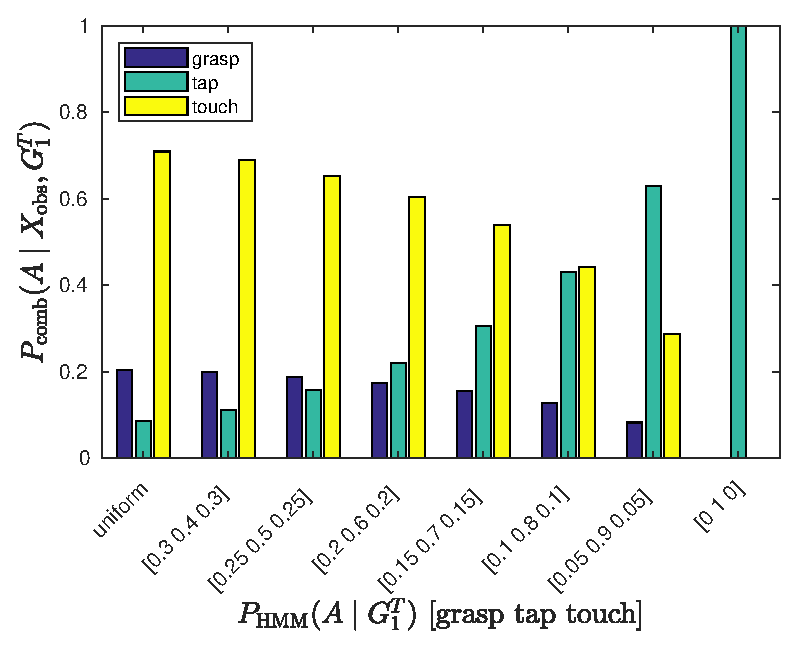
\includegraphics[width=0.9\columnwidth]{impact_of_evidence_on_Action.eps}
\caption{Affordances and gestures combined model: inference over action given the evidence $\xobs =\{\text{Size}=\text{small}, \text{Shape}=\text{sphere}, \text{ObjVel}=\text{slow}\}$, combined with different probabilistic soft evidence about the action.}
\label{fig:impact_of_evidence_on_Action}
\end{figure}

In this experiment, we test the ability of our approach to recognize actions.
Both the \AffWords{} model and the gesture recognizer can each perform inference of the action variable individually: the former by using the variables of Tab.~\ref{tab:salvi:bnsymb}, the latter by using human gesture features.
We show how our combined model performs the inference over action in a joint way.
This includes dealing with information with different degrees of confidence, or conflicting information.

Let us consider the evidence
$\xobs = \{$ Size=small, Shape=sphere, ObjVel=slow~$\}$.
This corresponds to an experiment that involves a small ball which, after the manipulative action, exhibits a low velocity.
Fig.~\ref{fig:impact_of_evidence_on_Action} displays the inference over the action variable by our model.

Based on the evidence, the affordance model alone gives the highest probability $\pbn(A \given \xobs)$ to the action \emph{touch}, which usually (in training) does not result in any movement of the object.
However, in this particular situation, let us further assume that the action performed by the human was an (unsuccessful) \emph{tap}, that is, a tap that does not result in any movement for the object.

In the figure, we show the effect of augmenting the inference with information from the gesture recognizer, that is, computing \eqref{eq:pcomb_inf_includes_action} (in the case where the action variable is included among the inference variables).
We analyze the effect of varying the degree of confidence of the gesture classifier.
We start from a uniform posterior $\phmm(A \given G_1^T)$, corresponding to a poor classifier, and gradually increase the probability of the correct action until it reaches~$1$.
In this particular example, in order to win the belief of the affordance model, the gesture recognizer needs to be very confident ($\phmm(A=\text{tap} \given G_1^T) > 0.81$).

\subsubsection{Inference over Effects}
\label{sec:gestures:results:affgest:inference_effects}

\begin{figure*}
\centering
\subfloat[][Predictions with a sphere object.]
{ 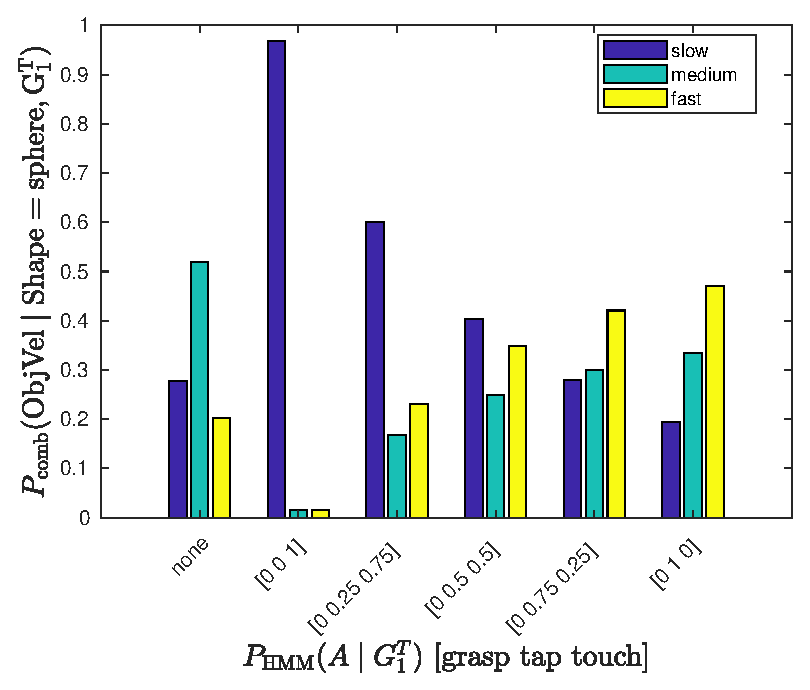
\includegraphics[width=0.45\linewidth]{impact_of_evidence_on_ObjVel_sphere.eps} \label{fig:impact_of_evidence_on_ObjVel_sphere} } \quad
%
\subfloat[][Predictions with a box object.]
{ 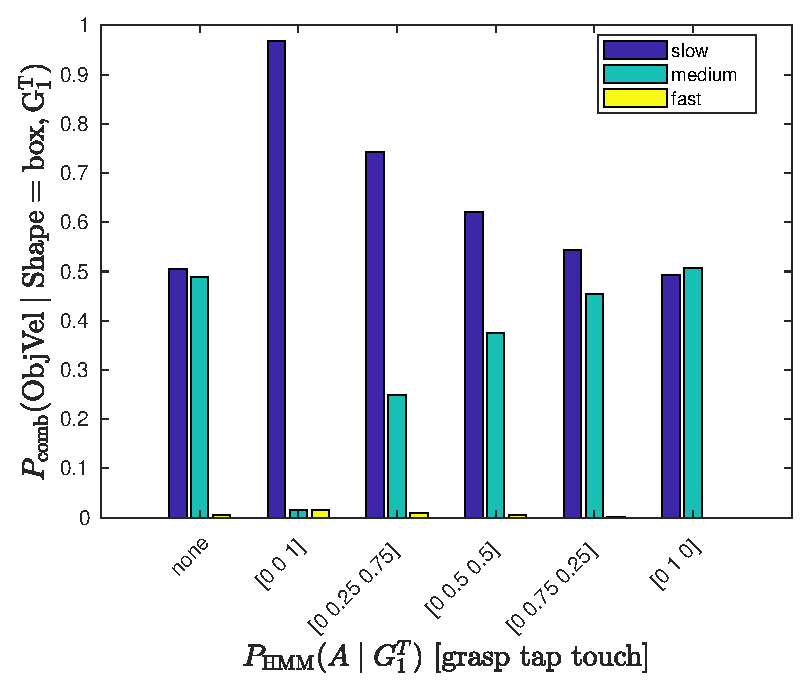
\includegraphics[width=0.45\linewidth]{impact_of_evidence_on_ObjVel_box.eps} \label{fig:impact_of_evidence_on_ObjVel_box} }
\caption{Affordances and gestures combined model: inference over the object velocity effect of different objects, when given probabilistic soft evidence about the action.}
\label{fig:impact_of_evidence_on_ObjVel}
\end{figure*}

We now show how our approach does inference over variables other than the action one.
This corresponds to computing \eqref{eq:pcomb_inf_excludes_action} (in the case where the action variable is not among the inference variables, but it is among the latent variables).

We will run this test by using different degrees of probabilistic confidence about the action, and analyzing the outcome in terms of velocity prediction.
This experiment exposes that \emph{all} the variables of Tab.~\ref{tab:salvi:bnsymb} jointly link robot and human, not only the action variable, for the reasons expressed in Sec.~\ref{sec:gestures:approach:affgest}.

Fig.~\ref{fig:impact_of_evidence_on_ObjVel} shows the considered inference in two cases: when the prior information indicates that the shape is spherical~(see Fig.~\ref{fig:impact_of_evidence_on_ObjVel_sphere}), and when it is cubic~(see Fig.~\ref{fig:impact_of_evidence_on_ObjVel_box}).

The leftmost distribution in both figures shows the prediction of object velocity from the \AffWords{} model alone, without any additional information.
When the shape is spherical, the model is not sure about the velocity, whereas if the shape is cubic, the model does not expect high velocities.
If we add clear evidence on the action \emph{touch} from the gesture recognizer, suddenly the combined model predicts slow velocities in both cases, as expected.
However, if the action recognition evidence is gradually changed from \emph{touch} to \emph{tap}, the predictions of the model depend on the shape of the object.
Higher velocities are expected for spherical objects that can roll, compared to cubic objects.

\subsubsection{Prediction of Word Probabilities}
\label{sec:gestures:results:affgest:prediction_words}

\begin{figure}
\centering
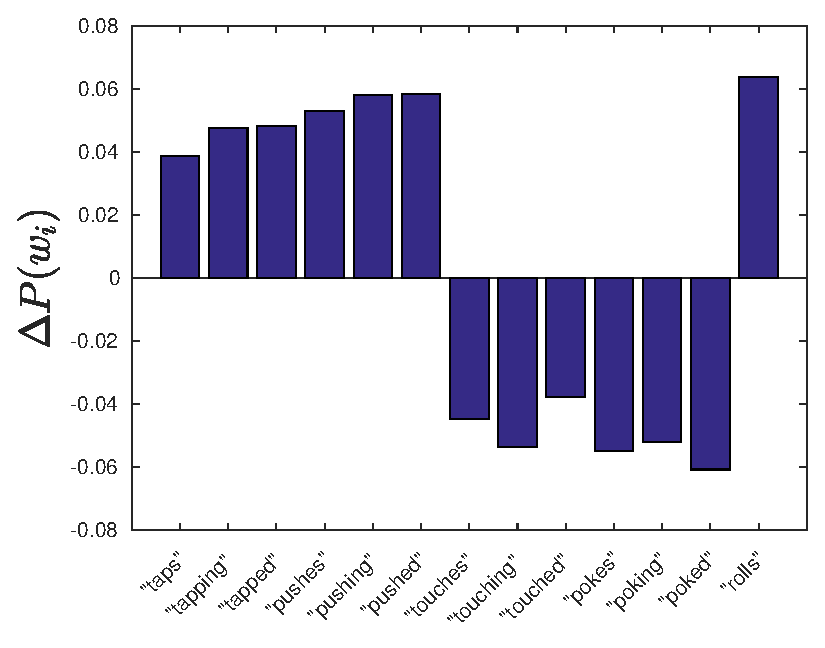
\includegraphics[width=0.9\columnwidth]{tcds-partialfig.eps}
\caption[Affordances and verbal language: variation of word occurrence probabilities.]{Affordances and verbal language: variation of word occurrence probabilities
$\Delta p(w_i) = \pcomb(w_i \given \xobs, \text{Action=tap}) - \pbn(w_i \given \xobs)$, where $\xobs = \{ \text{Size=big, Shape=sphere, ObjVel=fast} \}$.
This variation corresponds to the difference of word probability when we add the tap action evidence~(obtained from gesture recognition) to the initial evidence about object features and effects. We have omitted words for which no significant variation was observed.}
\label{fig:variation_word_occurrence_prob}
\end{figure}

Our model permits to make predictions over the word variables associated to affordance evidence (see Table~\ref{tab:salvi:bnsymb}, last row).
In Fig.~\ref{fig:variation_word_occurrence_prob} we show the variation in word occurrence probabilities between two cases:
\begin{enumerate}
\item when the robot's prior knowledge evidence consists of information about object features and effects only: \{Size=big, Shape=sphere, ObjVel=fast\};

\item when the evidence corresponds to the one of the previous point, with the addition of the \emph{tap} action observed from the gesture recognizer (deterministic hard evidence).
\end{enumerate}

This result is interesting for two reasons.
First, the probabilities of words related to tapping and pushing increase when a tapping action evidence from the gesture recognizer is introduced; conversely, the probabilities of other action words~(touching and poking) decreases.
Second, the probability of the word ``rolling''~(which is an effect of an action onto an object) also increases when the tap action evidence is entered.

\subsubsection{Effect Anticipation}
\label{sec:gestures:results:anticipation_effects}

\begin{figure*}
  \centering
  \subfloat[][Action performed on small sphere. Description: ``the robot pushed the ball and the ball moves''.]{
    \resizebox{0.9\linewidth}{!}{
      \begin{tikzpicture}
        \node (lik) {\includegraphics[width=0.6\linewidth]{evolution_of_action_posterior_sphere_log.eps}};
        \node at ([xshift=-90pt,yshift=30pt]lik.north) {\includegraphics[width=\myWidthTcds\linewidth]{tap-sphere-00000179}};
        \node at ([xshift=+10pt,yshift=30pt]lik.north) {\includegraphics[width=\myWidthTcds\linewidth]{tap-sphere-00000183}};
        \node at ([xshift=+110pt,yshift=30pt]lik.north) {\includegraphics[width=\myWidthTcds\linewidth]{tap-sphere-00000187}};
        \node at ([xshift=100pt,yshift=30pt]lik.east) {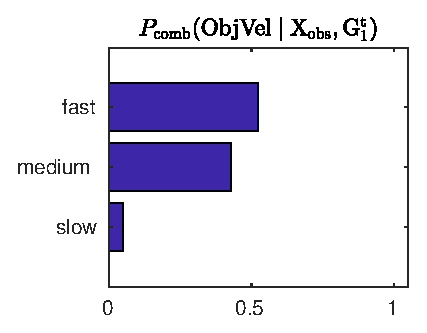
\includegraphics[width=0.35\linewidth]{evolution_of_action_posterior_sphere_effect_pred.eps}};
      \end{tikzpicture}
    } % end resizebox
    \label{fig:effect_pred_sphere}
  } % end subfloat

  \subfloat[][Action performed on big box. Description: ``the robot is pushing the big square but the box is inert''.]{
    \resizebox{0.9\linewidth}{!}{
      \begin{tikzpicture}
        \node (lik) {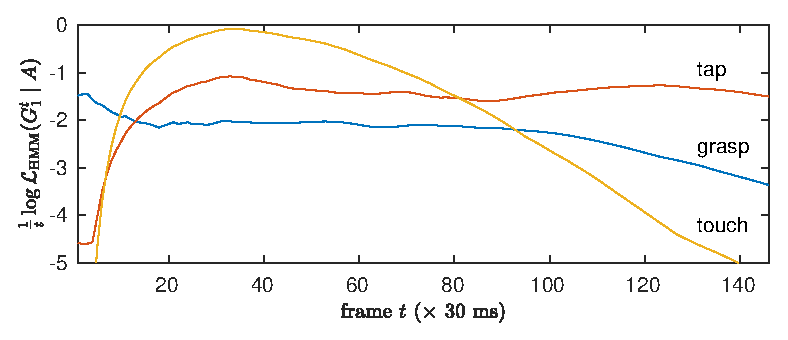
\includegraphics[width=0.6\linewidth]{evolution_of_action_posterior_box_log.eps}};
        \node at ([xshift=-90pt,yshift=30pt]lik.north) {\includegraphics[width=\myWidthTcds\linewidth]{tap-box-00000230}};
        \node at ([xshift=+10pt,yshift=30pt]lik.north) {\includegraphics[width=\myWidthTcds\linewidth]{tap-box-00000250}};
        \node at ([xshift=+110pt,yshift=30pt]lik.north) {\includegraphics[width=\myWidthTcds\linewidth]{tap-box-00000270}};
        \node at ([xshift=100pt,yshift=30pt]lik.east) {\includegraphics[width=0.35\linewidth]{evolution_of_action_posterior_box_effect_pred.eps}};
      \end{tikzpicture}
    } % end resizebox
  \label{fig:effect_pred_box}
  } % end subfloat
  \caption[Affordances and gestures combined model: object velocity effect anticipation before impact.]{Affordances and gestures combined model: object velocity effect anticipation before impact. The evidence from the gesture recognizer~(left) is fed into the \AffWords{} model before the end of the execution. The combined model predicts the effect~(right) and describes it in words~(verbal language).}
  \label{fig:effect_pred}
\end{figure*}

Since the gesture recognition method interprets sequences of human motions, we can test this predictive ability of our combined model when we observe an incomplete action.
Fig.~\ref{fig:effect_pred} shows an example of this where we reason about the expected object velocity caused by a tap action.

In particular, Fig.~\ref{fig:effect_pred_sphere} shows the action performed on a spherical object, whereas Fig.~\ref{fig:effect_pred_box} on a cubic one.
Within each of the two figures, the graphs on the left side show the time evolution of the evidence $\phmm(A \given G_1^t)$ from the gesture recognizer.
In order to make the variations emerge more clearly, instead of the posterior, we show $\frac{1}{t} \log \mathcal{L}_\text{HMM} (G_1^t \given A)$: the log-likelihood normalized by the length of the sequence.

Note how, in both cases, the correct action is recognized by the model given enough evidence, although the observation sequence is not complete.
The right side of the plot shows the prediction of the object velocity, given the incomplete observation of the action and the object properties.
The model correctly predicts that the sphere will probably move but the box is unlikely do so.
Finally, the captions in the figure also show the human-interpretable verbal description~(see Sec.~\ref{sec:gestures:approach:verbal}) generated by feeding the probability distribution of the words estimated by the model, given incomplete evidence, into the \ac{CFG}.

\subsection{Verbal Descriptions}
\label{sec:gestures:results:verbal}

We now present results about the verbal descriptions generated by the model with the \ac{CFG}.
They allow us to observe the emergence of non-trivial language phenomena (they emerge from our developmental model, not from the grammar itself, which is provided only for the purpose of interpreting the probability distributions over the words).

By generating and scoring verbal descriptions about what the robot observes~(see Sec.~\ref{sec:gestures:approach:verbal}), we can provide evidence to the model and interpret the verbal results.

From Sec.~\ref{sec:gestures:approach:verbal:descriptions} recall that, with our method, we do not add new words to the model when we observe the human performing actions.
Rather, the human-readable descriptions that we generate are based on the same words that were present in the self-centered learning phase (see Sec.~\ref{sec:gestures:approach:stages}).
In that phase, the verbal descriptions described the agent of the observed actions as either ``the~robot'', ``he'', or ``Baltazar''~(the name of the robot used in \cite{salvi:2012:smcb}).
Consequently, the \AffWords{} model learned by the robot includes those words as the subject of the action.

\subsubsection{Choice of Synonyms}
\label{sec:gestures:results:verbal:descriptions_and_synonyms}

\begin{table}
    \centering
    \caption{Affordances and verbal language: $10$-best list of sentences generated from the evidence $\xobs = \{ \text{Color=yellow, Size=big, Shape=sphere, ObjVel=fast} \}$.}
    \label{tab:example_generated_sentences}
    \resizebox{\linewidth}{!}{% https://tex.stackexchange.com/a/27105
    \begin{tabular}{ll}
    \toprule
    sentence & score \\
    \midrule
    ``the robot pushed the ball and the ball moves'' & $-0.54322$ \\
    ``the robot tapped the sphere and the sphere moves'' & $-0.5605$ \\
    ``he is pushing the sphere and the sphere moves'' & $-0.57731$ \\
    ``the robot is tapping the yellow ball and the big yellow sphere is moving'' & $-0.57932$ \\
    ``he pushed the yellow ball and the sphere is rolling'' & $-0.58853$ \\
    ``the robot is poking the ball and the sphere is rolling'' & $-0.58998$ \\
    ``he is pushing the ball and the yellow ball moves'' & $-0.59728$ \\
    ``he pushes the sphere and the ball is moving'' & $-0.60528$ \\
    ``he is tapping the yellow ball and the ball is moving'' & $-0.60675$ \\
    ``the robot pokes the sphere and the ball is rolling'' & $-0.60694$ \\
    \bottomrule
    \end{tabular}%
    } % end resizebox
\end{table}

As an example, by providing the evidence $\xobs=$\{Color=yellow, Size=big, Shape=sphere, ObjVel=fast\} to the model, we obtain the sentences reported in Table~\ref{tab:example_generated_sentences}.
The higher the score, the more likely the sentence.

In many of the sentences in the table, we note that
(i)~the correct verb related to the tap action is generated (in the initial evidence, no action information was present, only object features and effects information were), and
(ii)~the object term ``ball'' or synonyms thereof~(e.g., ``sphere'') are used coherently, both in the first part of the sentence describing the action and in the second part describing the effect.

This result shows that different synonyms may be used by the model in the same sentence.
This is a consequence of the random generation of sentences, described in Sec.~\ref{sec:gestures:approach:verbal:descriptions}, and because synonyms are often assigned similar (but not necessarily equal) probabilities by the model, given the same evidence.

\subsubsection{Choice of Conjunction}
\label{sec:gestures:results:verbal:conjunction}

The manipulation experiments that we consider in this chapter have the following structure, similar to the one described in Sec.~\ref{sec:platform:scenario}: an agent~(human or robot) performs a physical action onto an object with certain properties, and this object will show a certain physical effect as a result.
For example, a touch action on an object yields no physical movement, but a tap does~(especially if the object is spherical).
In the language description associated to an experiment, it makes sense to analyze the \emph{conjunction} chosen by the model given specific evidence.
In particular, it would be desirable to separate two kinds of behaviors: one in which the action and effect are coherent~(expected conjunction: ``and''), and the other one in which they are contradictory (``but'').

\newcommand{\evidenceProducingAnd}{$\xobs=$\{ Action=grasp, ObjVel=medium \}}
\newcommand{\evidenceProducingBut}{$\xobs=$\{ Action=grasp, ObjVel=slow \}}

\begin{figure*}
  \centering
  \subfloat[][Evidence: \evidenceProducingAnd.]{
    \begin{tabular}[b]{c}
    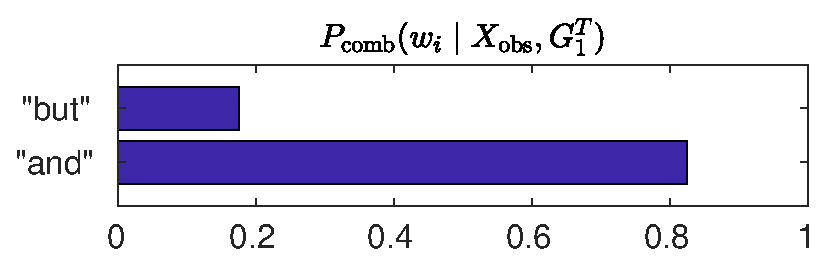
\includegraphics[width=0.4\linewidth]{p_conjunctions_and_evidence.eps}\\

    \resizebox{!}{0.1\linewidth}{% https://tex.stackexchange.com/a/27105
      \begin{tabular}{ll}
        \toprule
        sentence & score \\
        \midrule
        ``the robot is picking the sphere \textbf{and} the sphere is moving''  & $-0.59328$ \\
        ``the robot grasps the sphere \textbf{and} the ball is moving''  & $-0.59507$ \\
        ``the robot is picking the sphere \textbf{and} the sphere is rising''  & $-0.60882$ \\
        ``the robot grasped the sphere \textbf{and} the sphere is rising''  & $-0.61842$ \\
        ``the robot picked the ball \textbf{and} the ball is rising''  & $-0.64052$ \\
        ``baltazar grasps the sphere \textbf{and} the sphere is moving''  & $-0.66182$ \\
        ``the robot has grasped the ball \textbf{and} the ball is rising''  & $-0.66398$ \\
        ``the robot picked the ball \textbf{and} the green ball is moving''  & $-0.67134$ \\
        ``baltazar grasped the sphere \textbf{and} the ball is moving''  & $-0.67283$ \\
        ``baltazar is grasping the ball \textbf{and} the sphere is rising''  & $-0.6787$ \\
        \bottomrule
      \end{tabular}%
    } % end resizebox
    \end{tabular}
    \label{tab:conjunction:and}
  } % end subfloat
  \quad
  \subfloat[][Evidence: \evidenceProducingBut.]{
    \begin{tabular}[b]{c}
    \includegraphics[width=0.4\linewidth]{p_conjunctions_but_evidence.eps}\\

    \resizebox{!}{0.1\linewidth}{% https://tex.stackexchange.com/a/27105
      \begin{tabular}{ll}
        \toprule
        sentence & score \\
        \midrule
        ``the robot is picking the cube \textbf{but} the square is still''  & $-0.52575$ \\
        ``the robot is grasping the sphere \textbf{but} the box is inert''  & $-0.55$ \\
        ``the robot is grasping the square \textbf{but} the sphere is still''  & $-0.55388$ \\
        ``the robot grasped the square \textbf{but} the cube is inert''  & $-0.55608$ \\
        ``baltazar is grasping the square \textbf{but} the square is inert''  & $-0.5571$ \\
        ``the robot is grasping the cube \textbf{but} the ball is inert''  & $-0.56011$ \\
        ``the robot picks the box \textbf{but} the square is inert''  & $-0.56397$ \\
        ``baltazar is picking the square \textbf{but} the square is still''  & $-0.56402$ \\
        ``he is grasping the square \textbf{but} the cube is inert''  & $-0.56815$ \\
        ``the robot grasps the square \textbf{but} the sphere is inert''  & $-0.57417$ \\
        \bottomrule
      \end{tabular}%
    } % end resizebox
    \end{tabular}
    \label{tab:conjunction:but}
  } % end subfloat
    \caption[Affordances and verbal language: $10$-best list of sentences generated given two different sets of evidence.]%
    {Affordances and verbal language: $10$-best list of sentences generated given two different sets of evidence.
    In~(a) the model interprets the object movement as indicating a succesful grasp and uses the conjunction ``and''.
    In~(b) the slow movement is interpreted as no movement at all and, therefore, as an unsuccessful grasp: for that reason, the conjunction ``but'' is used.}
    \label{tab:conjunction}
\end{figure*}

Fig.~\ref{tab:conjunction} shows an example of the behavior described above.
We give the same action value \emph{grasp} to the model as evidence, but two different values for the final object velocity.
When the object velocity is medium~(Fig.~\ref{tab:conjunction:and}), the model interprets this as a successful grasp, and it uses the conjunction ``and'' to separate the description of the action from the description of the effect.
When the object velocity is slow~(in the clustering procedure, the velocity was most often zero in those cases), the model predicts that this is an unsuccessful grasp and it uses the conjunction ``but'', instead.

\subsubsection{Description of Object Features}
\label{sec:gestures:results:verbal:description_objects}

\newcommand{\graspBoxGreenOne}{``the robot is grasping the box and the green box is moving''}
\newcommand{\touchBoxGreenOne}{``the robot is poking the green square and the cube is inert''}
\newcommand{\graspSphereGreenTwo}{``the robot picked the ball and the green ball is moving''}
\newcommand{\touchSphereGreenTwo}{``baltazar is poking the green sphere and the sphere is still''}

\newcommand{\evidenceProducingGraspBoxGreenOne}{$\xobs = \{ \text{Action=grasp, Color=green1, Shape=box} \}$}
\newcommand{\evidenceProducingTouchBoxGreenOne}{$\xobs = \{ \text{Action=touch, Color=green1, Shape=box} \}$}
\newcommand{\evidenceProducingGraspSphereGreenTwo}{$\xobs = \{ \text{Action=grasp, Color=green2, Shape=sphere} \}$}
\newcommand{\evidenceProducingTouchSphereGreenTwo}{$\xobs = \{ \text{Action=touch, Color=green2, Shape=sphere} \}$}

\begin{figure}
  \centering
  \subfloat[][\graspBoxGreenOne.]{
    \resizebox{\linewidth}{!}{
      \includegraphics{graspBoxGreen1-00000007}
      \includegraphics{graspBoxGreen1-00000008}
      \includegraphics{graspBoxGreen1-00000009}
      \includegraphics{graspBoxGreen1-00000010}
      \includegraphics{graspBoxGreen1-00000013}
      \includegraphics{graspBoxGreen1-00000016}
    } % end resizebox
    \label{fig:verbal_descriptions:graspBoxGreenOne}
  } % end subfloat

  \subfloat[][\touchBoxGreenOne.]{
    \resizebox{\linewidth}{!}{
      \includegraphics{touchBoxGreen1-00000008}
      \includegraphics{touchBoxGreen1-00000009}
      \includegraphics{touchBoxGreen1-00000010}
      \includegraphics{touchBoxGreen1-00000011}
      \includegraphics{touchBoxGreen1-00000013}
      \includegraphics{touchBoxGreen1-00000015}
    } % end resizebox
    \label{fig:verbal_descriptions:touchBoxGreenOne}
  } % end subfloat

  \subfloat[][\graspSphereGreenTwo.]{
    \resizebox{\linewidth}{!}{
      \includegraphics{graspSphereGreen2-00000007}
      \includegraphics{graspSphereGreen2-00000008}
      \includegraphics{graspSphereGreen2-00000009}
      \includegraphics{graspSphereGreen2-00000011}
      \includegraphics{graspSphereGreen2-00000013}
      \includegraphics{graspSphereGreen2-00000015}
    } % end resizebox
    \label{fig:verbal_descriptions:graspSphereGreenTwo}
  } % end subfloat

  \subfloat[][\touchSphereGreenTwo.]{
    \resizebox{\linewidth}{!}{
      \includegraphics{touchSphereGreen2-00000006}
      \includegraphics{touchSphereGreen2-00000007}
      \includegraphics{touchSphereGreen2-00000008}
      \includegraphics{touchSphereGreen2-00000010}
      \includegraphics{touchSphereGreen2-00000011}
      \includegraphics{touchSphereGreen2-00000012}
    } % end resizebox
    \label{fig:verbal_descriptions:touchSphereGreenTwo}
  } % end subfloat

  \caption{Affordances and verbal language: examples of descriptions generated by the model.}
  \label{fig:verbal_descriptions}
\end{figure}

In Fig.~\ref{fig:verbal_descriptions}, we show examples of verbal descriptions generated by the model given different values of observed evidence:
\begin{itemize}
\item \evidenceProducingGraspBoxGreenOne{} (Fig.~\ref{fig:verbal_descriptions:graspBoxGreenOne});

\item \evidenceProducingTouchBoxGreenOne{} (Fig.~\ref{fig:verbal_descriptions:touchBoxGreenOne});

\item \evidenceProducingGraspSphereGreenTwo{} (Fig.~\ref{fig:verbal_descriptions:graspSphereGreenTwo});

\item \evidenceProducingTouchSphereGreenTwo{} (Fig.~\ref{fig:verbal_descriptions:touchSphereGreenTwo}).
\end{itemize}
Note that the box object in the two first examples has a dark shade of green~(value of Color affordance variable of Table~\ref{tab:salvi:bnsymb} clustered as:~green1), whereas the spherical one in the two last examples has a lighter shade (Color value:~green2).
However, the verbal descriptions reported in Fig.~\ref{fig:verbal_descriptions} all use the adjective ``green''.
This behavior emerges from fact that the robot develops its perceptual symbols (clusters) in an early phase, and only subsequently associates them with the human vocabulary.
We believe that this phenomenon is practical and potentially useful~(i.e., the possibility that a low-level fine-grained robot representation can be abstracted into a high-level language description, which bundles the two shades of green under the same word).

\section{Conclusions and Future Work}
\label{sec:gestures:conclusions}

This chapter has illustrated a computational model that combines object affordances, human gestures and verbal language.
We presented such a combined model, allowing a robot to interpret and describe the actions of external agents, by reusing the knowledge previously acquired in an ego-centric manner.

We have shown that for cognitive robots it is possible, and indeed fruitful, to combine knowledge acquired from interacting with elements of the environment~(affordances) with the probabilistic observation of another agent's actions~(gestures) as well as verbal language elements.
In this sense, our model supports the growing field of \emph{\hr{} collaboration}~\cite{bauer:2008:ijhr,dragan:2015:hri}, whose goal is to enable effective teamwork between humans and robots.

In a developmental setting, the robot learns the link between words and object affordances by exploring its environment.
Then, it classifies the manipulative gestures performed by another agent.
Finally, by fusing the information from the affordances model and a gesture recognizer, the robot can reason over affordances and words when observing the other agent.
This can also be leveraged to do early action recognition~(see Sec.~\ref{sec:gestures:results:anticipation_effects}).

In terms of language, although the complete model only estimates probabilities of single words given the evidence, we showed that feeding these probabilities into a pre-defined grammar produces human-interpretable sentences that correctly describe the situation.
We also highlighted some interesting language-related properties of the combined model, such as:
the choice of relevant words to describe a scene,
the choice of synonyms,
and of congruent/incongruent conjunctions,

Our demonstrations are based on a restricted scenario~(see Sec.~\ref{sec:gestures:related:salvi}), i.e., one human and one robot manipulating simple objects on a shared table, a pre-defined number of motor actions and effects, and a vocabulary of approximately~$50$ words to describe the experiments verbally.
However, one of the main strengths of our study is that it spans different fields such as robot learning, language grounding, and object affordances.
We also work with real robotic data, as opposed to learning images-to-text mappings~(as in many works in computer vision) or using robot simulations~(as in many works in robotics).

In terms of \emph{scalability}, note that our \ac{BN} model can learn both the dependency structure and the parameters of the model from observations.
The method that estimates the dependency structure, in particular, is sensitive to biases in the data.
Consequently, in order to avoid misconceptions, the robot needs to explore any possible situation that may occur.
For example, if the robot only observes blue spheres rolling and the objects with any other shape are never blue, it might infer that it is the color that makes the object roll, rather than its shape.
In order to scale the method to a larger number of concepts, it would be necessary to scale the amount of data considerably, similarly to what is done in many deep learning approaches.
In models of developmental robotics, where this is neither practically feasible, nor desirable, we would need to devise methods that can generalize more efficiently from very few observations.

As future work, it would be useful to investigate how the model can extract syntactic information from the observed data autonomously, thus relaxing the bag-of-words assumption in the current model.
Another line of research would be to study how the model can guide the discovery of new acoustic patterns~(e.g., \cite{falstrom:2017:glu, vanhainen:2014:icassp, vanhainen:2012:interspeech}), and how to incorporate the newly discovered symbols into our \AffWords{} model.
This would release our current assumption of a pre-defined set of words.
